\documentclass{article}

% Pacotes Utilizados -----------------------------------------------------------
\usepackage[brazil]{babel}
\usepackage[utf8]{inputenc}
\usepackage[T1]{fontenc}
\usepackage{graphicx}
\usepackage{sbc-template}

% Informações Pessoais ---------------------------------------------------------

\begin{document}

O presente documento apresenta o Relatório sobre desenvolvimento de calculadora
didática, solicitada como Projeto Prático GB1 desta disciplina. Utilizando um
circuito integrado 74LS381, as operações solicitadas foram implementadas. Para
exibir os valores de entrada e saída, houve a necessidade de implementação de um
\emph{display} de 7 segmentos e um conjunto de multiplexadores para exibição dos
dois valores de entrada e único de saída.

Portanto, durante a construção, podemos dividir o conjunto de componentes em
três módulos distintos: a apresentação do conteúdo num \emph{display} de 7
segmentos, seletor de entradas no \emph{display} utilizando um conjunto de
multiplexadores e aplicação das operações solicitadas no circuito integrado em
questão.

% Display de 7 Segmentos -------------------------------------------------------
\section{\emph{Display} de 7 Segmentos}

Para visualizar os valores apresentados como entradas ao circuito integrado
responsável pelos cálculos aritméticos e lógicos, bem como seu valor resultante
na saída, precisamos criar um módulo para exibição destes valores num
\emph{display} de 7 segmentos.

Para isto, utilizamos o circuito integrado 74LS47N que recebe como parâmetros de
entrada os 4 valores binários e apresenta como saída 7 valores que devem ser
apresentados ao \emph{display}. Para evitar posteriores ruídos ocorridos durante
a implementação da calculadora didática, precisamos aplicar um resistor de
470ohms em cada entrada do circuito integrado. O diagrama elétrico pode ser
visualizado conforme Figura \ref{fig:ci7447}.

\begin{figure}
    \centering{}
    \includegraphics[width=\textwidth]{ci7447.ps}
    \caption{Circuito Elétrico para \emph{Display} de 7 Segmentos}
    \label{fig:ci7447}
\end{figure}

Como podemos visualizar, o circuito possui 4 entradas A3 até A0 que serão
consideradas como entradas do módulo do \emph{display}. Podemos então exibir o
módulo de forma mais genérica conforme Figura \ref{fig:s-ci7447}.

\begin{figure}
    \centering{}
    \includegraphics[scale=0.3,angle=270]{s-ci7447.ps}
    \caption{Circuito Elétrico para \emph{Display} de 7 Segmentos Simplificado}
    \label{fig:s-ci7447}
\end{figure}

% Multiplexadores --------------------------------------------------------------
\section{Multiplexadores}

Para exibir os dois valores de entrada e único de saída no mesmo \emph{display},
resultantes dos cálculos aritméticos e lógicos, precisamos utilizar 3 circuitos
integrados multiplexadores 74LS157 que irão receber como 3 entradas de 4
\emph{bits} dos valores que devem ser exibidos.

Para seleção do valor que deverá ser exibido no \emph{display} de 7 segmentos,
vamos utilizar os seletores disponíveis em cada multiplexador, direcionando
assim a saída desejada para o módulo de exibição. O diagrama elétrico pode ser
visualizado conforme Figura \ref{fig:ci74157}.

\begin{figure}
    \centering{}
    \includegraphics[width=\textwidth]{ci74157.ps}
    \caption{Circuito Elétrico para Multiplexadores}
    \label{fig:ci74157}
\end{figure}

Como podemos visualizar, as entradas A e B que serão apresentadas ao circuito
integrado responsável pelo processamento aritmético e lógico devem também ser
apresentadas para este módulo, assim como o resultado do processamento deve ser
adicionado na entrada F desta estrutura. A exibição é dada conforme os sinais
que são apresentados às entradas S0 e S1. Quando S0 e S1 estão em nível baixo, a
saída é dada para a entrada A; quando S0 está em nível alto e S1 em nível baixo,
a saída é atribuída para a entrada B; e quando S1 está em nível alto,
independendo do valor de S0, a saída é dada para o valor apresentado em F da
estrutura.

Com o desenvolvimento deste módulo, podemos representá-lo com uma estutura mais
simples e concatená-lo à estrutura responsável pelo \emph{display} de 7
segmentos, conforme Figura \ref{fig:s-ci74157-ci7447}.

\begin{figure}
    \centering{}
    \includegraphics[scale=0.5,angle=270]{s-ci74157-ci7447.ps}
    \caption{Circuito Elétrico para Multiplexadores com \emph{Display}
        Simplificado}
    \label{fig:s-ci74157-ci7447}
\end{figure}

% Calculadora Didática ---------------------------------------------------------
\section{Calculadora Didática}

Agora que temos a estrutura básica de exibição de entradas e saída em
\emph{display}, podemos desenvolver o módulo para execução de cálculos
aritméticos e lógicos, utilizando o circuito integrado 74LS381, uma ULA de 4
\emph{bits}.

Utilizando \emph{dip switches}, vamos conectar as entradas A e B no circuito
integrado de cálculos e nos multiplexadores, que também irão receber a saída
resultante. Também serão conectados aos \emph{dip switches} os 2 valores
seletores de visualização no \emph{display}, bem como os 3 valores seletores de
função a ser executada sobre os dados de entrada, disponíveis no circuito
responsável pelos cálculos. O diagrama elétrico pode ser visualizado na Figura
\ref{fig:ci74381}.

\begin{figure}
    \centering{}
    \includegraphics[width=\textwidth]{ci74381.ps}
    \caption{ULA 4 \emph{bits} com Multiplexadores e \emph{Display}}
    \label{fig:ci74381}
\end{figure}

Conforme a figura apresentada, existem 3 conjuntos de \emph{dip switches}
responsáveis pelo controle do circuito. O \emph{dip switch} D2 é responsável
pelo controle das funcionalidades do circuito, onde os dois primeiros manipulam
os multiplexadores e os demais as funções da ULA. Os \emph{dip switches} D1 e D0
são responsáveis pelas entradas A e B, respectivamente. Porém, o pino 1 de D0 é
responsável pelo \emph{carry} que deve ser informado quando uma subtração está
selecionada.

\end{document}

